%%% Kapitel "uber die Anwendung 'meiner' k.p Methode auf geordnetes GaInP
%%% Time-stamp: <1999-03-04 11:50:00 ralf>

%%%%%%%%%%%%%%%%%%%%%%%%%%%%%%%%%%%%%%%%%%%%%%%%%%%%%%%%%%%%%%
%%%%%%%%%%%%%%%%%%%%%%%%%%%%%%%%%%%%%%%%%%%%%%%%%%%%%%%%%%%%%%
%%%%
%%%%
\chapter{Anwendung auf geordnetes \GaInP}
\label{cha:anwend}

In diesem Kapitel soll gezeigt werden, wie sich die in
Kap.~\ref{cha:period-stoer} abgeleitete Theorie auf ein konkretes Problem, die
effektive Masse der Elektronen im Leitungsband von (teil-)geordnetem \GaInP,
anwenden l"a"st.

%%%%%%%%%%%%%%%%%%%%%%%%%%%%%%%%%%%%%%%%%%%%%%%%%%%%%%%%%%%%%%
%%%%
\section{Allgemeines zum Materialsystem}
\label{sec:materialsystem}

Viele III--V-Halbleiterlegierungen $A_{x}B_{1-x}C$ mit Kationen $A$ und $B$
zeigen spontane, langreichweitige \CuPt-Ordnung, wenn sie mit
metallorganischer Gasphasen-Epitaxie [\emph{metalorganic vapour phase epitaxy}
(MOVPE)] auf $(001)$-orientierten Substraten gewachsen werden \cite{zuma:94}.
Die geordnete Phase besteht aus abwechselnden Monolagen
$A_{x+\eta/2}B_{1-x-\eta/2}C$ und $A_{x-\eta/2}B_{1-x+\eta/2}C$, die l"angs
der $[111]$-Richtung angeordnet sind. Dabei ist $0 \le \eta \le 1$ der
Ordnungsgrad. Die $[111]$-Richtung wird als Ordnungsrichtung
bezeichnet.\footnote{Im Prinzip w"are auch eine der drei Richtungen m"oglich,
  die zur $[111]$-Richtung "aquivalent sind. Doch hat dies hier keinerlei
  Auswirkungen, so da"s wir hier bei nur einer Richtung bleiben wollen.}

Ein prominentes Beispiel f"ur diese Materialien ist
Ga$_{x}$In$_{1-x}$P. Mit \GaInP\ wollen wir den Fall $x \approx 0.5$
bezeichnen, der gitterangepa"st auf GaAs Substraten aufgewachsen werden kann
\cite{kipp:97}. Ein Vergleich der mikroskopischen Struktur der ungeordneten
Zinkblende-Struktur und einem \CuPt-geordneten Material ist in
Abb.~\ref{fig:ZnS-CuPt} zu sehen.

\begin{figure}[hbtp]
  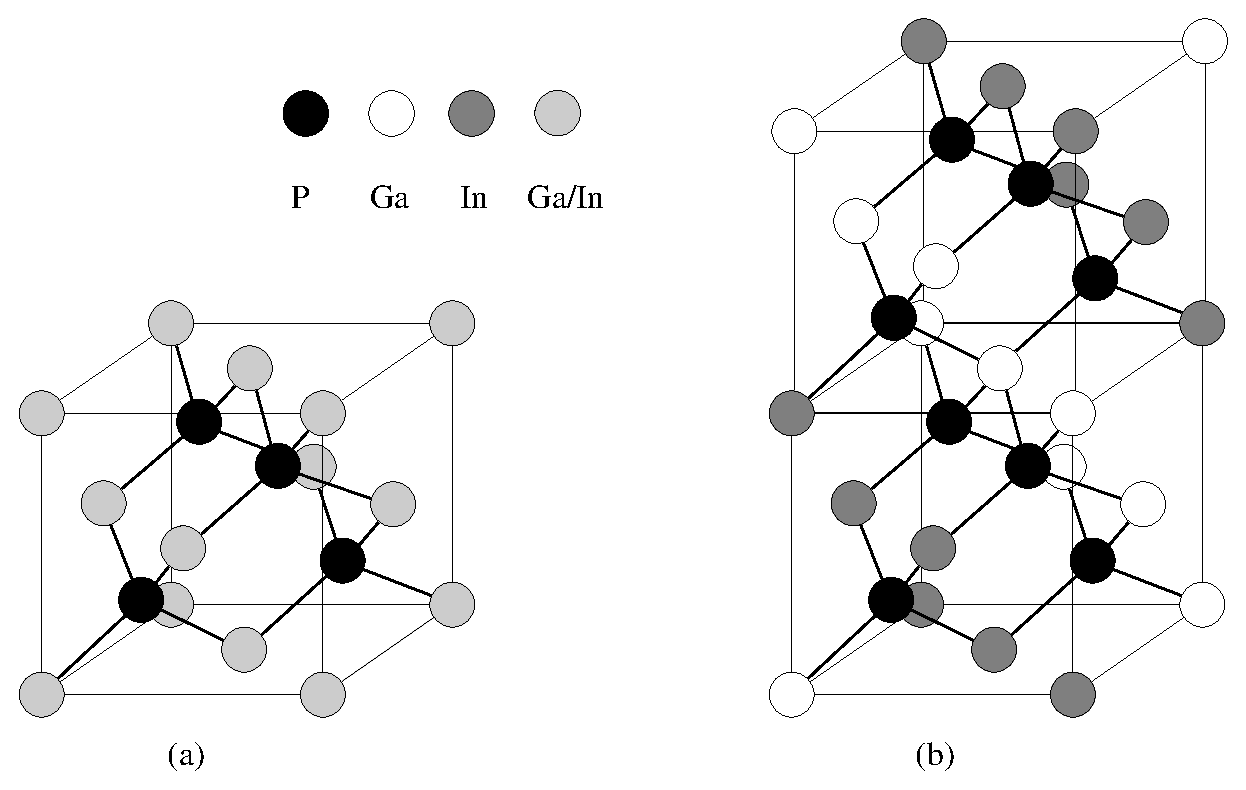
\includegraphics[width=\textwidth]{zns.eps}
  \caption{Vergleich der mikroskopischen Struktur in einem (a)
    Zinkblende-Gitter mit einem (b) vollst"andig \CuPt-geordneten Material.}
  \label{fig:ZnS-CuPt}
\end{figure}

Abb.~\ref{fig:ZnS-CuPt}(b) zeigt den Fall idealer Ordnung, d.~h.\
Ordnungsgrad $\eta=1$. Allerdings wurden im Experiment bisher nur teilgeordnete
Proben gefunden. Das bedeutet $\eta < 1$, so da"s auf  aufeinanderfolgenden
$(111)$-Ebenen die \emph{Wahrscheinlichkeit} abwechselnd erh"oht (erniedrigt)
und erniedrigt (erh"oht) ist, ein Ga (In) Atom zu finden. Dabei h"angt der
Ordnungsgrad von verschiedenen Wachstumsbedingungen wie Temperatur und
Substratorientierung ab.

%\begin{floatingfigure}{50mm}
%  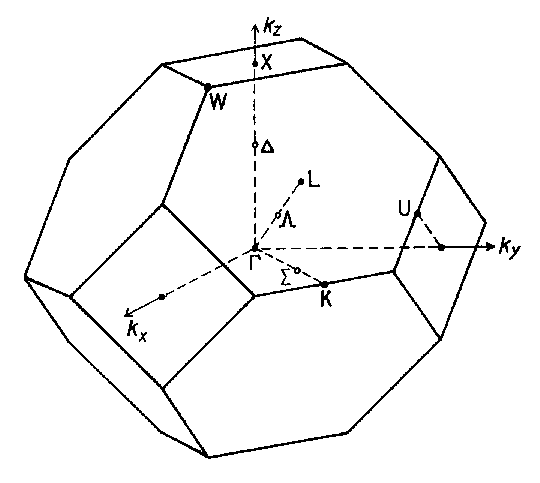
\includegraphics[width=40mm]{bz-fcc.eps}
%  \caption{Brillouin Zone eines Zinkblende Kristalls}
%  \label{fig:bz-fcc}
%\end{floatingfigure}


\begin{floatingfigure}{75mm}
  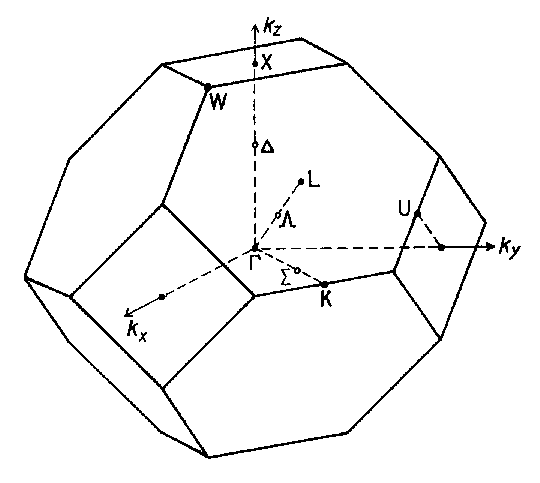
\includegraphics[width=65mm]{bz-fcc.eps}
  \caption{Brillouin Zone eines Kristalls mit Zinkblende-Struktur}
  \label{fig:bz-fcc}
\end{floatingfigure}


\sloppy 
Beim "Ubergang vom unge"-ordneten ($\eta=0$) Zinkblende-System zu einem
\CuPt-ge"-ordneten Kristall wird die Einheitszelle verdoppelt und damit die
Brillouin-Zone halbiert. Die Punktgruppe des Kristalls reduziert sich von \Td\ 
zu \Cdv.\footnote{Die Bezeichnungen von Punktgruppen und derer (irreduziblen)
  Darstellungen folgt der Notation von Koster \emph{et al.}  \cite{kdws:63}.}
Diese Verkleinerung der Brillouin-Zone bewirkt ein Zur"uckfalten von
Zust"anden. An jedem Punkt der neuen Brillouin-Zone finden sich Zust"ande, die
sich urspr"unglich an zwei verschiedenen Punkten der Brillouin-Zone des
Zinkblende-Gitters befanden. Die f"ur uns interessanten Zust"ande befinden
sich im Zentrum der neuen Brillouin-Zone.  Der eine Teil der dort zu findenden
Zust"ande war auch im Zinkblende-Gitter schon am $\Gamma$-Punkt. Der andere
Teil faltet von dem L-Punkt zur"uck, der in Ordnungsrichtung
liegt.\footnote{Den vier prinzipiell m"oglichen Ordnungsrichtungen entsprechen
  auch vier L-Punkte.}
%Der Satz \set\ an Punkten im reziproken Raum umfa"st hier also den $\Gamma$-
%und den L-Punkt.

\fussy

Dies f"uhrt zu einer ganzen Reihe von Effekten, von denen wir die wichtigsten
hier behandeln wollen. Zwei der auff"alligsten  
sind die Reduzierung der Bandl"ucke um $\Delta E_{\text{BGR}}$ und die
Kristallfeldaufspaltung $\Delta_{\text{CF}}$. Letzteres bedeutet, da"s das ohne
Spin-Bahn-Wechselwirkung dreifach entartete \GVB-Valenzband"-maximum in einen
zweifach entarteten $\bGVB{3} (\GVB)$-Zustand und einen einfach entarteten
$\bGVB{1} (\GVB)$-Zustand aufspaltet.\footnote{Bei der Notation der Zust"ande
  in der teilgeordneten Phase, folgen wir hier der z.~B.\ in
  Ref.~\cite{wfz:95} zu findenden. Dabei wird die Symmetrie eines Zustandes im
  \CuPt-geordneten Kristall mit einem Strich versehen, w"ahrend die Symmetrie
  desjenigen Zinkblende-Zustands der ma"sgeblich beitr"agt in Klammern
  angegeben wird. Die Zuordnung der Zinkblende-Zust"ande ist
  Abb.~\ref{fig:band-short} zu entnehmen.}

%\begin{figure}[htb]
%  \begin{minipage}[c]{50mm}
%    \caption{Brillouin-Zone eines Kristalls mit Zinkblende-Struktur}
%    \label{fig:bz-fcc}
%  \end{minipage}
%  \hfill
%  \begin{minipage}[c]{70mm}
%    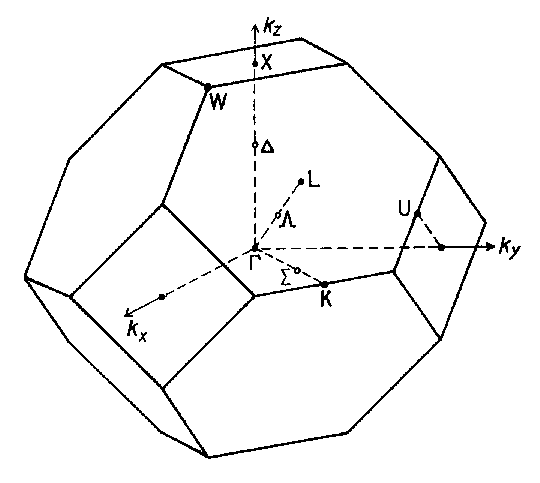
\includegraphics[width=70mm]{bz-fcc.eps}
%  \end{minipage}
%\end{figure}

Wird die Spin-Bahn-Wech"-sel"-wirkung ber"ucksichtigt, so zeigt sich die
Kristallfeldaufspaltung in einer Aufhebung der vierfachen Entartung des
$\Gamma_{\text{8v}}$ Valenzbandes. Die sich hier ergebende Aufspaltung
entspricht \emph{nicht} der Kristallfeldaufspaltung. Aus der
Valenzbandaufspaltung l"a"st sich aber die Kristallfeldaufspaltung berechnen,
wenn f"ur die Spin-Bahn-Wechselwirkung die quasikubische N"aherung gemacht
wird \cite{bipi:74}, bei der eine von der Symmetrie her m"ogliche Anisotropie
in der Spin-Bahn-Wechselwirkung vernachl"assigt wird. 

Theoretische Vorhersagen \cite{wezu:98} und Messungen \cite{fzcm:97,fgmz:98}
haben gezeigt, da"s zwischen Bandl"uckenreduzierung $\Delta E_{\text{BGR}}$ und
Kristallfeldaufspaltung $\Delta_{\text{CF}}$ eine vom Ordnungsgrad
unabh"angige Beziehung herrscht. F"ur \GaInP\ finden diese Autoren
%
\begin{equation}
  \label{eq:zeta}
  \zeta_{\text{theo}} = \frac{\Delta E_{\text{BGR}}}{\Delta_{\text{CF}}} = 2,69
  \quad \text{bzw.} \quad \zeta_{\text{exp}} \approx 2,65 .
\end{equation}
%

Weiterhin sind in (teil-)geordnetem \GaInP\ optische "Uberg"ange m"oglich, die
im ungeordneten Fall dipolverboten sind. Einer von diesen ist der "Ubergang
$\bGVB{3}(\GVB) \rightarrow \bGCB (\LCB)$, der vor kurzem genauer
untersucht wurde \cite{kksk:99}. Tr"agt man die "Ubergangsenergie als Funktion der
Bandl"uckenreduzierung auf, so ergibt sich eine Gerade mit Steigung
$\theta = 0,48$. Es besteht also ein eindeutiger Zusammenhang zwischen dem
Ordnungsgrad, repr"asentiert durch die Bandl"uckenreduzierung $\Delta
E_{\text{BGR}}$, und der "Anderung $\Delta E_{\Gamma \rightarrow \text{L}}$
der Energie des "Ubergang $\bGVB{3}(\GVB) \rightarrow \bGCB (\LCB)$, gegeben
durch 
%
\begin{equation}
  \label{eq:theta}
  \theta = \frac{\Delta E_{\Gamma \rightarrow \text{L}}}
  {\Delta E_{\text{BGR}}} = 0,48 .
\end{equation}
%
%Diese beiden Zahlen werden in Kap.~\ref{sec:betrag} wichtig sein,
%wenn es darum geht, den Betrag von Matrixelementen zu bestimmen.


%%%%%%%%%%%%%%%%%%%%%%%%%%%%%%%%%%%%%%%%%%%%%%%%%%%%%%%%%%%%%%
%%%%
\section{Beschreibung der effektiven Massen im Leitungsband}
\label{sec:k.p-m-CB}

Die bisher erw"ahnten Untersuchungen besch"aftigten sich nur mit den Energien
verschiedener Zust"ande in Abh"angigkeit vom Ordnungsgrad, d.~h.\ mit
statischen Eigenschaften. Eine wichtige Gr"o"se bei der Beschreibung
dynamischer Eigenschaften -- z.~B.\ Transportph"anomenen -- sind die
effektiven Massen der Elektronen im Valenz- und Leitungsband.
%\marginpar{Etwas "uber die Definition
%  der effektiven Masse???}

Als erste versuchten Raikh und Tsiper \cite{rats:94}, die effektive Masse im
Leitungsband "uber die Kopplung zwischen den B"andern \GCB\ und \LCB\ im
Rahmen einer Effektive-Massen-N"aherung zu beschreiben. Das unbekannte
Matrixelement f"ur diese Kopplung pa"sten sie dabei an beobachtete
Bandl"uckenreduzierungen an, da \LCB\ energetisch h"oher liegt als \GCB\ und
die Kopplung zu einer Absto"sung dieser Zust"ande f"uhrt. Au"serdem mischen
die Zust"ande auf Grund dieser Kopplung. Da die effektiven Massen von \LCB\ 
anisotrop und gr"o"ser als bei \GCB\ sind, ergibt sich mit diesem Modell die
Vorhersage eines Anstiegs der effektiven Masse im untersten Leitungsband als
Funktion des Ordnungsgrades.  Dabei sollte der Anstieg parallel zur
Ordnungsrichtung gr"o"ser sein als senkrecht zu ihr, also
$m^{\ast}_{\parallel} > m^{\ast}_{\perp} > m^{\ast}_{\text{c}}$. Hier
bezeichnet $m^{\ast}_{\text{c}}$ die isotrope effektive Masse von \GCB,
$m^{\ast}_{\parallel}$ die effektive Masse parallel zur Ordnungsrichtung und
$m^{\ast}_{\perp}$ die effektive Masse senkrecht zur Ordnungsrichtung.

Problematisch bei diesem Ansatz ist, da"s die Bandl"uckenreduzierung zu einer
Verst"arkung der Wechselwirkung zwischen Valenzbandmaximum und
Leitungsbandminimum f"uhrt, was eine \emph{Reduzierung} der effektiven Masse
im Leitungsband zur Folge hat. Dies wurde von Zhang und Mascarenhas
\cite{zhma:95} untersucht. Ausgehend von einem acht B"ander
($\Gamma_{\text{6c}}, \Gamma_{\text{8v}}, \Gamma_{\text{7v}}$) umfassenden
\kdotp-Hamilton-Operator f"ur den ungeordneten Kristall, ber"ucksichtigten sie
die Ordnungseffekte durch zwei Parameter, welche die Bandl"uckenreduzierung
und Kristallfeldaufspaltung beschreiben.\footnote{Tats"achlich f"uhren sie
  zun"achst mehr Parameter ein, deren Form sich aus Symmetrie"uberlegungen
  ergibt, vernachl"assigen dann aber die "Ubrigen.}  Sie erhielten damit eine
reduzierte effektive Masse im Leitungsband. Bedingt durch die
Kristallfeldaufspaltung im Valenzband fiel diese in Ordnungsrichtung
schw"acher aus, also $m^{\ast}_{\text{c}} > m^{\ast}_{\parallel} >
m^{\ast}_{\perp}$.

In diesem Ansatz fehlen aber die Effekte der $\Gamma$--L-Mischung, die
nicht vernachl"assigbar sind. Franceschetti, Wei und Zunger \cite{fwz:95}
zeigten dies, indem sie \emph{ab initio} Bandstruktur-Rechnungen
(Dichtefunktionaltheorie in lokaler Dichten"aherung) f"ur den ideal
geordneten Fall durchf"uhrten. Dabei fanden sie $m^{\ast}_{\parallel} >
m^{\ast}_{\perp}$, in "Ubereinstimmung mit obigen Rechnungen. Aber die
effektive Masse im ungeordneten Material befand sich zwischen diesen beiden
Werten, also $m^{\ast}_{\parallel} > m^{\ast}_{\text{c}} > m^{\ast}_{\perp}$.
Die Schlu"sfolgerung der Autoren war, da"s die effektive Masse der
Leitungsbandelektronen empfindlich davon abh"angt, in welchem Verh"altnis
$\Gamma$--L-Mischung und verst"arkte Kopplung zum Valenzband zueinander
stehen.

Sowohl die $\Gamma$--L-Mischung, als auch die verst"arkte Kopplung zum
Valenzband beruhen beide auf der Wechselwirkung zwischen Zinkblende
$\Gamma$- und L-Zust"anden. Ein Modell, das diese Wechselwirkung richtig
beschreibt, sollte deshalb auch in der Lage sein, die Ordnungsabh"angigkeit
der effektiven Masse im Leitungsband korrekt zu beschreiben. Ein solches
Modell ist mit der in Kap.~\ref{cha:period-stoer} abgeleiteten Theorie
m"oglich, und wir wollen sie nun auf dieses Problem anwenden.


%%%%%%%%%%%%%%%%%%%%%%%%%%%%%%%%%%%%%%%%
\subsection{Wahl der Basisfunktionen}
\label{sec:basiswahl}

Das ungest"orte Problem von dem wir ausgehen wollen ist der ungeordnete
Kristall, beschrieben durch den Hamilton-Operator \op{H_{0}}. F"ur diesen
ben"otigen wir als Parameter die Energieeigenwerte $\veps_{n}(\vec{k})$ und
die Impulsmatrixelemente \pnnK\ aus Gl.~\eqref{eq:h0}. Dazu f"uhren wir eine
Bandstruktur-Rechnung durch und beschreiben dabei den ungeordneten Kristall
mit der N"aherung eines virtuellen Kristalls [\emph{virtual crystal
  approximation} (VCA)]. F"ur diese Berechnung verwenden wir die Methode der
Linearkombination atomarer Orbitale [\emph{linear combination of atomic
  orbitals} (LCAO), oft auch \emph{tight-binding approximation} (TBA)
genannt]. Dabei bleibt die Spin-Bahn-Wechselwirkung unber"ucksichtigt. Die
Spin-Bahn-Aufspaltung ist mit einem Betrag von etwa 100~meV verglichen mit
einer Bandl"ucke von 1.97~eV nicht vernachl"assigbar, doch ist der Einflu"s
der Spin-Bahn-Aufspaltung auf die effektive Masse im Leitungsband sehr gering.
Auf Details dieser Rechnung werden wir in Anhang \ref{cha:lcao} eingehen.
Ergebnisse sind z.~B.\ in Abb.~\ref{fig:band-short} dargestellt.

\begin{figure}[htb]
  \includegraphics[width=\textwidth]{band-short.eps}
  \caption{Bandstruktur in ungeordnetem \GaInP}
  \label{fig:band-short}
\end{figure}


Die St"orung \op{H_{1}} entspricht dem Unterschied zwischen dem
Kristallpotential im (teil-)geordneten und ungeordneten Fall. Dieses
Ordnungspotential\footnote{Dieser Begriff wurde zuerst von Wei und Zunger
  \cite{wezu:89} eingef"uhrt.}  
hat nicht mehr die Symmetrie des Zinkblende-Gitters (Punktgruppe \Td) sondern
die der geordneten Phase, f"ur die \CuPt-Struktur also Punktgruppe \Cdv.
Deshalb ist es in der Lage, Zust"ande verschiedener Symmetrie im
Zinkblende-Gitter zu koppeln, wenn sie in der \CuPt-geordneten Struktur die
gleiche Symmetrie haben. Dabei wollen wir nur Kopplungen zwischen Zust"anden
ber"ucksichtigen, die zu verschiedenen \vec{k}-Punkten im Zinkblende-Kristall
geh"oren, aber nach der Faltung am gleichen \vec{k}-Punkt zu finden sind. Das
bedeutet, da"s in der Entwicklung \eqref{eq:h1-Gm} nur diejenigen
Koeffizienten $\rho_{m}$ ber"ucksichtigt werden, die zu \emph{neuen}
reziproken Gittervektoren \nG\ geh"oren, aber nicht die, die zu alten
reziproken Gittervektoren \aG\ geh"oren. Raikh und Tsiper
\cite{rats:94} haben gezeigt, da"s dies im Rahmen der VCA exakt gilt, wenn im
geordneten Kristall keine Relaxationen auftreten. Experimente, welche das Ma"s
an Relaxation untersuchten, wurden bisher nicht ver"offentlicht.  Theoretische
Untersuchungen \cite{wfz:95,ylcy:97} lassen keinen eindeutigen Schlu"s zu,
ob Relaxationen notwendig sind oder nicht, um beobachtete Gr"o"sen wie z.~B.\ 
die Kristallfeldaufspaltung zu erkl"aren. Allerdings stimmen sie darin
"uberein, da"s Relaxationen auch die Kopplung zwischen Zust"anden von
verschiedenen \vec{k}-Punkten der Zinkblende-Brillouin-Zone verst"arken
w"urden, so da"s es gerechtfertigt erscheint, die Matrixelemente zwischen
Zust"anden vom gleichen \vec{k}-Punkt zu vernachl"assigen. F"ur die in
Kap.~\ref{sec:disk} skizzierte Matrixform des Hamilton-Operators hei"st dies,
da"s die \VnnKKee\ und \VnnKKzz\ nicht ber"ucksichtigt werden.

Wie in Kap.~\ref{sec:basis} gezeigt, sind die Zust"ande von $\Gamma$- und
L-Punkt, die hier den Satz \{\set\} aus Kap.~\ref{sec:basis} bilden,
ein vollst"andiges Orthonormalsystem. Doch ist das sich daraus ergebende
unendlich-dimensionale Gleichungssystem f"ur praktische Rechnungen nicht
praktikabel, weshalb die Einschr"ankung auf eine geeignete Basis ein wichtiger
Schritt ist. Die kleinste Basis, die es noch erm"oglicht die
wesentlichen physikalischen Vorg"ange zu beschreiben, enth"alt die Zust"ande
\GCB, \GVB, \LCB\ und \LVB\ (siehe Abb.~\ref{fig:band-short}). Zwischen den
Leitungsbandzust"anden ist auf Grund des geringen Energieabstandes eine starke
Wechselwirkung zu erwarten. Die Mischung dieser Zust"ande beeinflu"st die
effektiven Massen im Leitungsband unmittelbar. Zus"atzlich reduziert sich noch
die Bandl"ucke, was die \kdotp-Wechselwirkung mit dem Valenzband verst"arkt.
Um dies zu beschreiben, reicht es aber nicht aus, nur die \GVB-Zust"ande zu
ber"ucksichtigen, da die Kristallfeldaufspaltung zu einer Anisotropie in der
\kdotp-Wechselwirkung zwischen Valenz- und Leitungsband f"uhrt. Die
Kristallfeldaufspaltung k"onnen wir aber nur "uber die Wechselwirkung zwischen
\GVB- und \LVB-Zust"anden erkl"aren, so da"s die \LVB-Zust"ande auch in die
Basis aufgenommen werden m"ussen.



%%%%%%%%%%%%%%%%%%%%%%%%%%%%%%%%%%%%%%%%
\subsection{Der \kdotp-Hamilton-Operator}
\label{sec:k.p-H}

Die Form des \kdotp-Hamilton-Operators, der zur Basis aus
Kap.~\ref{sec:basiswahl} geh"ort, l"a"st sich aus allgemeinen
gruppentheoretischen "Uberlegungen ableiten. Dabei wollen wir zun"achst die
Standard \kdotp\ Teile betrachten.

Der \kdotp-Hamilton-Operator f"ur \GCB\ und \GVB\ ist wohlbekannt.
Vernachl"assigen wir das Fehlen von Inversionssymmetrie und w"ahlen $x$, $y$
und $z$ entlang der kubischen Kristallachsen $[100]$, $[010]$ und $[001]$, so
ist er durch 
%Gl.~\eqref{eq:k.p-G} 
%
%\setcounter{floateq}{\value{equation}}
%\begin{floateq}
\vspace*{4ex}
\begin{equation}
\renewcommand{\arraystretch}{1.6}
\setlength{\arraycolsep}{0.5ex}
\label{eq:k.p-G}
\op{H_{\Gamma}} = 
\left(
\begin{array}{c|ccc}
  \raisebox{2.0em}[0ex][0ex]{\ket{\GCB}} 
& \raisebox{2.0em}[0ex][0ex]{\ket{\GVBx}} 
& \raisebox{2.0em}[0ex][0ex]{\ket{\GVBy}} 
& \raisebox{2.0em}[0ex][0ex]{\ket{\GVBz}} \\[-4ex]
%%%%%%%%%%% 
\begin{array}[c]{c}
 E_{\Gamma\text{c}} + \frac{\hbar^{2}}{2m} k^{2} \\ + \pri{A} k^{2}  
\end{array}
&  i\PG k_{x} 
&  i\PG k_{y} 
&  i\PG k_{z} \\
%%%%%%%%%%%
\hline
  -i\cc{\PG} k_{x} 
& \begin{array}[c]{c}
  \frac{\hbar^{2}}{2m} k^{2} + \pri{L} k_{x}^{2} \\ 
  + \pri{M} (k_{y}^{2}+k_{z}^{2})
\end{array}
& \pri{N} k_{x} k_{y} 
& \pri{N} k_{x} k_{z} \\
%%%%%%%%%%%
  -i\cc{\PG} k_{y} 
& \pri{N} k_{x} k_{y} 
& \begin{array}[c]{c}
  \frac{\hbar^{2}}{2m} k^{2} + \pri{L} k_{y}^{2} \\ 
  + \pri{M} (k_{x}^{2}+k_{z}^{2})
\end{array}
& \pri{N} k_{y} k_{z} \\
%%%%%%%%%%%
  -i\cc{\PG} k_{z} 
& \pri{N} k_{x} k_{z} 
& \pri{N} k_{y} k_{z} 
& \begin{array}[c]{c}
  \frac{\hbar^{2}}{2m} k^{2} + \pri{L} k_{z}^{2} \\ 
  + \pri{M} (k_{x}^{2}+k_{y}^{2})
\end{array} \\
\end{array}\right) 
\renewcommand{\arraystretch}{0.625}
\end{equation}
%\end{floateq}
%
gegeben \cite{kane:66}, wobei $\pri{A}$, $\pri{L}$, $\pri{M}$ und $\pri{N}$
die Wechselwirkung mit energetisch weiter entfernten B"andern repr"asentieren,
die "uber L"owdin-St"orungstheorie \cite{lowd:51} ber"ucksichtigt wurde; $m$
ist die Masse des freien Elektrons. Das reduzierte Impulsmatrixelement \PG\ 
ist gegeben durch
%
\begin{displaymath}
  \PG = - i \frac{\hbar}{m} \matrixel{\GCB}{\op{p_{x}}}{\GVBx}.
\end{displaymath}
%
Dieses Matrixelement bezieht sich dabei auf ein Integral "uber die
Einheitszelle von ungeordnetem \GaInP\ von der Form \eqref{eq:pnnK}. Dort
entspricht der Integrationsbereich zwar der Einheitszelle von geordnetem
\GaInP, doch wie bereits in Kap.~\ref{sec:h0} erw"ahnt, h"angt der Wert des
Impulsmatrixelements nicht vom Integrationsbereich ab, da sich das auftretende
Normierungsvolumen entsprechend "andert.

Der Hamilton-Operator f"ur das \LVB-Band ist z.~B.\ bei Bir und
Pikus~\cite{bipi:74} zu finden, wobei wiederum Terme linear in \vec{k}, die
von der Inversionsasymmetrie des Zinkblende-Gitters herr"uhren,
vernachl"assigt werden. Wir wollen aber die Wechselwirkung mit \LCB\ explizit
ber"ucksichtigen, so da"s wir untersuchen m"ussen, welche Impulsmatrixelemente
zwischen diesen Zust"anden existieren. W"ahlen wir die $z$-Achse parallel zur
$[111]$-Richtung, so transformiert sich die $z$-Komponente des Impulsoperators
gem"a"s der irreduziblen Darstellung \IRREP{1} von \Cdv, $x$- und
$y$-Komponente wie \IRREP{3}. Das Wigner-Eckart-Theorem zusammen mit den bei
Koster \emph{et al.} \cite{kdws:63} tabellierten Clebsch-Gordan-Koeffizienten
ergibt nun, da"s es am L-Punkt, "ahnlich wie am $\Gamma$-Punkt, nur ein
reduziertes Impulsmatrixelement innerhalb der von uns gew"ahlten Basis gibt.
Im Unterschied zum $\Gamma$-Punkt gibt es aber keine Kopplung in $z$-Richtung,
da $\matrixel{\LCB}{\op{p}_{z}}{\LVB} = 0 $ gilt.\footnote{In der Sprache der
  Gruppentheorie hei"st das, da"s \IRREP{1} nicht in der Produktdarstellung
  $\IRREP{1} \otimes \IRREP{3}$ enthalten ist.}  Somit erhalten wir
%Gl.~\eqref{eq:k.p-L}
%
%\setcounter{floateq}{\value{equation}}
%\begin{floateq}
  \vspace*{4ex}
\begin{equation}
\label{eq:k.p-L}
\renewcommand{\arraystretch}{1.6}
\setlength{\arraycolsep}{0.5ex}
\op{H_{\text{L}}} = \left(
\begin{array}{c|cc}
  \raisebox{2.0em}[0ex][0ex]{\ket{\LCB}} 
& \raisebox{2.0em}[0ex][0ex]{\ket{\LVBx}} 
& \raisebox{2.0em}[0ex][0ex]{\ket{\LVBy}} \\[-4ex]
%%%%%%%%%%%
\begin{array}[c]{c}
  E_{\text{Lc}} + \frac{\hbar^{2}}{2m} k^{2} \\ 
  + F k_{\perp}^{2} + G k_{z}^{2} 
\end{array}
& i\PL k_{x} 
& i\PL k_{y} \\
\hline
%%%%%%%%%%%
  -i\cc{\PL} k_{x} 
& \begin{array}[c]{c}
  E_{\text{Lv}} + \frac{\hbar^{2}}{2m} k^{2} + A k_{z}^{2} \\
  + B (k_{x}^{2}+k_{y}^{2}) + C k_{y} k_{z}
\end{array}
& C k_{x} k_{z} \\
%%%%%%%%%%%
  -i\cc{\PL} k_{y} 
& C k_{x} k_{z} 
& \begin{array}[c]{c}
  E_{\text{Lv}} + \frac{\hbar^{2}}{2m} k^{2} + A k_{z}^{2} \\ 
  + B (k_{x}^{2}+k_{y}^{2}) + C k_{y} k_{z}
\end{array}\\
\end{array}\right),
\renewcommand{\arraystretch}{0.625}
\end{equation}
%\end{floateq}
%
wobei $A$, $B$, $C$, $F$ und $G$ die Wechselwirkung mit energetisch weiter
entfernten B"andern beschreiben. Das reduzierte Impulsmatrixelement \PL\ ist
gegeben durch
%
\begin{displaymath}
  \PL =  - i \frac{\hbar}{m} \matrixel{\LCB}{\op{p_{x}}}{\LVBx}.
\end{displaymath}
%
Dabei wurde neben $\ez \parallel [111]$ noch $\ex \parallel [1 \bar{1} 0]$ und
$\ey \parallel [1 1 \bar{2}]$ gew"ahlt. Da dann $x$ in einer Spiegelebene von
\Cdv\ liegt, $y$ dagegen senkrecht zu dieser steht, erkl"art dies die
$x$-$y$-Asymmetrie in Gl.~\eqref{eq:k.p-L}.
 
\begin{figure}[htb]
  \includegraphics[width=\textwidth]{band-long.eps}
  \caption{Bandstruktur in ungeordnetem \GaInP. Senkrecht zur $[111]$-Richtung
    ist die Dispersion am L-Punkt qualitativ "ahnlich zu der am
    $\Gamma$-Punkt.} 
  \label{fig:band-long}
\end{figure}

Damit wir bei der Bestimmung der m"oglichen Potentialmatrixelemente das
Wigner-Eckart-Theorem effektiv anwenden k"onnen, m"ussen wir
Gl.~\eqref{eq:k.p-G} im gleichen Koordinatensystem wie Gl.~\eqref{eq:k.p-L}
schreiben. Da wir hier nicht versuchen wollen, die Dispersion der
Valenzb"ander zu beschreiben, brauchen wir die Parameter $\pri{L}$, $\pri{M}$
und $\pri{N}$ in Gl.~\eqref{eq:k.p-G} nicht zu ber"ucksichtigen, wodurch die
n"otige Drehung des Koordinatensystems f"ur die Hamilton-Matrix
\eqref{eq:k.p-G} trivial wird. Aus den selben Gr"unden k"onnen wir auch $A$,
$B$ und $C$ in Gl.~\eqref{eq:k.p-L} vernachl"assigen. 

Es ist bekannt, da"s im Zentrum der Brillouin-Zone die effektive Masse des
untersten Leitungsbandes zum gr"o"sten Teil "uber die Wechselwirkung mit dem
Valenzbandmaximum erkl"art werden kann. Dabei stammt der zweitgr"o"ste Anteil
von der Wechselwirkung mit dem untersten sich nach \IRREP{5} transformierenden
Leitungsband. Das mit dieser Wechselwirkung assoziierte Matrixelement
\pri{\PG} (siehe Abb.~\ref{fig:short+V_P}) betr"agt aber etwa $0.35 \PG$
\cite{ccf:88} und soll deshalb hier vernachl"assigt werden. Wir w"ahlen also
$\pri{A}=0$ in der Hamilton-Matrix \eqref{eq:k.p-G}.

In Abb.~\ref{fig:band-long} ist zu sehen, da"s die Dispersion am L-Punkt
\emph{senkrecht} zur $[111]$-Richtung qualitativ "ahnlich zu der am
$\Gamma$-Punkt ist. Auch die Beziehung zwischen \pri{\PL} und \PL\ ist
vergleichbar zu der von \pri{\PG} und \PG, wie Cardona zeigen konnte
\cite{card:63}. Deshalb wollen wir auch diesen Fernbandbeitrag
vernachl"assigen und damit in Gl.~\eqref{eq:k.p-L} $F=0$ w"ahlen.

\renewcommand{\bottomfraction}{0.7}
%
\begin{figure}[hb]
  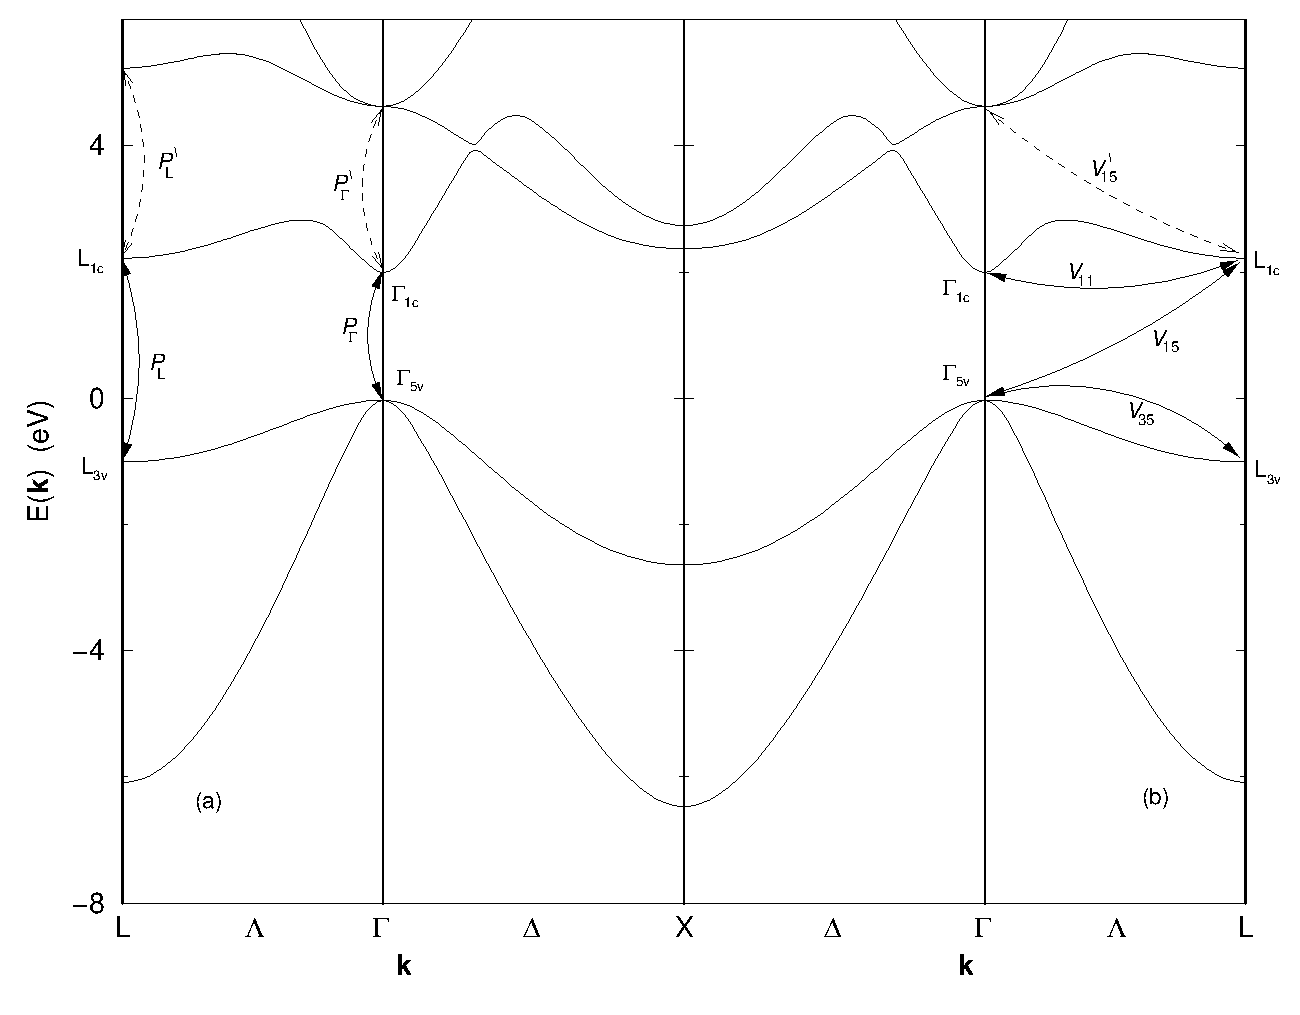
\includegraphics[width=\textwidth]{short+V_P.eps}
  \caption{Bandstruktur in  ungeordnetem GaInP mit (a) \kdotp- und (b)
      Potential-Matrixelementen.} 
  \label{fig:short+V_P}
\end{figure}
%

Nur die Dispersion am L-Punkt parallel zur $[111]$-Richtung l"a"st sich nicht
mit Wechselwirkungen innerhalb der hier gew"ahlten Basis erkl"aren. Deshalb
behalten wir $G$ als einzigen Beitrag energetisch weiter entfernter B"ander in
unserem Modell.

Die Bestimmung der m"oglichen Potentialmatrixelemente ist direkt "uber das
Wigner-Eckart Theorem m"oglich.\footnote{Da sich \op{H_{1}} gem"a"s der
  trivialen Darstellung \IRREP{1} von \Cdv\ transformiert, kann auch eine
  spezielle Form des Wigner-Eckart-Theorems verwendet werden \cite{corn:69}.
  Diese besagt, da"s dann nur Matrixelemente zwischen Zust"anden m"oglich
  sind, die sich nach der gleichen irreduziblen Darstellung
  transformieren, und die dazugeh"origen Clebsch-Gordan-Koeffizienten
  proportional zur Einsmatrix sind.}  
\LCB\ und \op{H_{1}} transformieren sich gem"a"s \IRREP{1} von \Cdv, \LVBx\ 
und \LVBy\ transformieren sich gemeinsam gem"a"s \IRREP{3}. Die
Wellenfunktionen des $\Gamma$-Punkts haben ein wohldefiniertes
Transformationsverhalten unter den Operationen von \Td. Uns interessiert aber,
wie sie sich unter Transformationen von \Cdv\ verhalten. Da \Cdv\ eine
Untergruppe der \Td\ ist, l"a"st sich diese Frage mit Hilfe der
Kompatibilit"atsrelationen beantworten, wie sie bei Koster \emph{et al.}
\cite{kdws:63} zu finden sind. Mit dem bei Gl.~\eqref{eq:k.p-L} verwendeten
Koordinatensystem erhalten wir, da"s sich \GCB\ und \GVBz\ gem"a"s \IRREP{1}
von \Cdv\ transformieren, und da"s \GVBx\ und \GVBy\ sich gemeinsam gem"a"s
\IRREP{3} von \Cdv\ transformieren. Damit ergibt sich, da"s es nur drei
verschiedene Matrixelemente zwischen den Zust"anden in unserer Basis gibt:
%
\begin{subequations}
\label{eq:def-V}
\begin{eqnarray}
\label{eq:V11,V35,V15}
  \V{11} &=& \matrixel{\GCB}{\op{H_{1}}}{\LCB}\\
  \V{35} &=& \matrixel{\GVBx}{\op{H_{1}}}{\LVBx} =
  \matrixel{\GVBy}{\op{H_{1}}}{\LVBy} \\
  \V{15} &=& \matrixel{\GVBz}{\op{H_{1}}}{\LCB}
\end{eqnarray}
\end{subequations}
%
Dabei bezieht sich das Matrixelement auf ein Integral "uber die Einheitszelle
von geordnetem \GaInP\ von der Form \eqref{eq:VnnKK}. Ordnungsbedingte
Wechselwirkungen mit Zust"anden au"serhalb der hier gew"ahlten Basis werden
wegen des gro"sen energetischen Abstands dieser Niveaus nicht ber"uchsichtigt.

Abb.~\ref{fig:short+V_P} zeigt nochmal im "Uberblick, welche Matrixelemente in
unserem Modell ber"ucksichtigt werden (durchgezogenen Linien). Als
durchbrochene Linien sind noch diejenigen Impuls- und Potentialmatrixelemente
eingezeichnet, die bei einer Verfeinerung des Modells als erste
ber"ucksichtigt werden sollten.

%
%%%%%%%%%%%% Gesamt k.p Hamilton-Operator
\begin{sidewaysfloateqnum}
\begin{equation}
\label{eq:k.p-H}
\caption{\kdotp-Hamilton-Operator inklusive Potentialmatrixelementen}
\renewcommand{\arraystretch}{1.6}
\op{H_{\Gamma \text{L}}} = \left(
\begin{array}{c|cc|c||c|cc}
  \raisebox{2.0em}[0ex][0ex]{\ket{\GCB}} 
& \raisebox{2.0em}[0ex][0ex]{\ket{\GVBx}} 
& \raisebox{2.0em}[0ex][0ex]{\ket{\GVBy}} 
& \raisebox{2.0em}[0ex][0ex]{\ket{\GVBz}} 
& \raisebox{2.0em}[0ex][0ex]{\ket{\LCB}} 
& \raisebox{2.0em}[0ex][0ex]{\ket{\LVBx}} 
& \raisebox{2.0em}[0ex][0ex]{\ket{\LVBy}} \\[-4ex]
%%%%%%%%%%%
E_{\Gamma\text{c}} + \frac{\hbar^{2}}{2m} k^{2} 
& i\PG k_{x} 
& i\PG k_{y} 
& i\PG k_{z} 
& \V{11} 
& 0 
& 0 \\
\hline
%%%%%%%%%%%
  -i\cc{\PG} k_{x} 
& \frac{\hbar^{2}}{2m}k ^{2} 
& 0 
& 0 
& 0 
& \V{35} 
& 0 \\
%%%%%%%%%%%
  -i\cc{\PG} k_{y} 
& 0 
& \frac{\hbar^{2}}{2m} k^{2} 
& 0 
& 0 
& 0 
& \V{35}   \\
%%%%%%%%%%%
\hline
  -i\cc{\PG} k_{z} 
& 0 
& 0 
& \frac{\hbar^{2}}{2m} k^{2} 
& \V{15} 
& 0 
& 0 \\
\hline\hline
%%%%%%%%%%%
\cc{\V{11}} 
& 0 
& 0 
& \cc{\V{15}} 
& \begin{array}[c]{c} E_{\text{Lc}} + \frac{\hbar^{2}}{2m} k^{2}\\
  + G k_{z}^{2}
  \end{array} 
& i\PL k_{x} 
& i\PL k_{y}\\
%%%%%%%%%%%
\hline
0 
& \cc{\V{35}} 
& 0 
& 0 
& -i\cc{\PL} k_{x} 
& E_{\text{Lv}} + \frac{\hbar^{2}}{2m} k^{2} 
& 0 \\
%%%%%%%%%%%
0 
& 0 
& \cc{\V{35}} 
& 0 
& -i\cc{\PL} k_{y} 
& 0 
& E_{\text{Lv}} + \frac{\hbar^{2}}{2m} k^{2} \\
\end{array} \right)
\renewcommand{\arraystretch}{0.625}
\end{equation}
\end{sidewaysfloateqnum}
%
Fassen wir nun Gln.~\eqref{eq:k.p-G} und \eqref{eq:k.p-L} mit diesem Ergebnis
zusammen, so erhalten wir als Hamilton-Operator Gl.~\eqref{eq:k.p-H} (siehe
S.~\pageref{eq:k.p-H}). Dabei haben wir die oben genannten N"aherungen
bez"uglich der Fernbandbeitr"age bereits ber"ucksichtigt.

%%%%%%%%%%%%%%%%%%%%%%%%%
% Betrag und Phase der Matrixelemente

%%%%%%%%%%%%%%%%%%%%%%%%%%%%%%%%%%%%%%%%%%%%%%%%%%%%%%%%%%%%%%
%%%%
\section{Bestimmung der Matrixelemente}
\label{sec:ME}

Um Gl.~\eqref{eq:k.p-H} l"osen zu k"onnen, ist es notwendig, die in ihr
vorkommenden Matrixelemente zu bestimmen. Eine wichtige Voraussetzung dazu
ist, da"s wir sowohl am $\Gamma$- als auch am L-Punkt eines Zinkblende-Gitters
die Wellenfunktionen reell w"ahlen k"onnen, wenn wir -- wie hier geschehen --
keine Spin-Bahn-Wechselwirkung ber"ucksichtigen. Dieser Effekt der
Zeitumkehrsymmetrie soll im folgenden kurz erl"autert werden.

Sei $\psi_{n\vec{k}}$ eine L"osung der station"aren Schr"odinger-Gleichung,
d.~h.\ 
%
\begin{displaymath}
    \op{H} \psi_{n\vec{k}} = \veps_{n}(\vec{k})\psi_{n\vec{k}},
\end{displaymath}
%
f"ur das Problem eines Teilchens in einem periodischen Potential. In diesem
Fall gilt das Bloch-Theorem
%
\begin{equation}
  \label{eq:Bloch-Theorem}
  \psi_{n\vec{k}}(\vec{r} + \vec{R}) = e^{i\sprod{k}{R}} \psi_{n\vec{k}}(\vec{r})
\end{equation}
%
f"ur alle Gittervektoren $\vec{R}$ des periodischen Potentials. Der
Wellenvektor \vec{k} h"angt also mit der diskreten Translationsinvarianz des
Problems zusammen. Ist \op{H} zeitumkehrinvariant, so ist aber auch
$\cc{\psi}_{n\vec{k}}$ ein L"osung der station"aren Schr"odinger-Gleichung zum
gleichen Eigenwert:\footnote{Betrachtet man die (zeitabh"angige)
  Schr"odinger-Gleichung, so sieht man, da"s die komplex-konjugierte Gleichung
  als zeitumgekehrte Gleichung aufgefa"st werden kann. F"ur einen
  zeitumkehrinvarianten Hamiltonoperator gilt also $\cc{\op{H}}=\op{H}$. Die
  Eigenwerte sind reell, da \op{H} hermitesch ist.}
%
\begin{displaymath}
  \op{H} \cc{\psi}_{n\vec{k}} = \veps_{n}(\vec{k}) \cc{\psi}_{n\vec{k}}
\end{displaymath}
%
Bilden wir nun das komplex-konjugierte von Gl.~\eqref{eq:Bloch-Theorem},
so erhalten wir
%
\begin{displaymath}
  \cc{\psi}_{n\vec{k}}(\vec{r} + \vec{R}) = e^{-i\sprod{k}{R}}
  \cc{\psi}_{n\vec{k}}(\vec{r}) ,
\end{displaymath}
%
d.~h.\ $\cc{\psi}_{n\vec{k}}$ geh"ort zum Wellenvektor \vec{-k}. Am
$\Gamma$-Punkt sind aber wegen $k=0$ sowohl $\psi_{n\vec{k}}$ als auch
$\cc{\psi}_{n\vec{k}}$ am gleichen Punkt im reziproken Raum angesiedelt.
F"ur den L-Punkt mit $\vec{k} = 2\pi/a_{\text{latt}} (1/2,1/2,1/2)$ gilt das
ebenso, da $-\vec{k} = \vec{k}- \vec{G}$ mit dem reziproken Gittervektor
$\vec{G} = 2\pi/a_{\text{latt}} (1,1,1)$ gilt, und somit
%
\begin{displaymath}
  \cc{\psi}_{n\vec{k}}(\vec{r} + \vec{R}) = 
  e^{-i\sprod{k}{R}} \cc{\psi}_{n\vec{k}}(\vec{r}) =
  e^{i\sprod{(k-G)}{R}} \cc{\psi}_{n\vec{k}}(\vec{r}) =
  e^{i\sprod{k}{R}} \cc{\psi}_{n\vec{k}}(\vec{r}),
\end{displaymath}
%
wegen $\sprod{G}{R}=2\pi n$ und $n \in \mathbb{Z}$ f"ur alle Gittervektoren
\vec{G} und \vec{R} des reziproken und realen Raumes. Wenn aber sowohl
$\psi_{n\vec{k}}$ als auch $\cc{\psi}_{n\vec{k}}$ Eigenzust"ande zum gleichen
Energie-Eigenwert und zum gleichen Wellenvektor sind, so k"onnen wir immer
reelle Funktionen $\frac{1}{2}(\psi_{n\vec{k}} + \cc{\psi}_{n\vec{k}})$ und
$\frac{1}{2i}(\psi_{n\vec{k}} - \cc{\psi}_{n\vec{k}})$ verwenden. Wir k"onnen
also davon ausgehen, da"s wir es in unserer Basis nur mit reellen
Wellenfunktionen zu tun haben. Dies bedeutet aber f"ur die in \op{H_{\Gamma
\text{L}}} [Gl.~\eqref{eq:k.p-H}] auftretenden Matrixelemente, da"s sie
ebenfalls reell sind. 


%%%%%%%%%%%%%%%%%%%%%%%%%%%%%%%%%%%%%%%%
\subsection{Betrag der Matrixelemente}
\label{sec:betrag}

F"ur $\V{11} = \V{35} = \V{15} = 0$ beschreibt Gl.~\eqref{eq:k.p-H}
den ungeordneten Kristall, den wir im Rahmen der TBA modellieren (siehe
Anhang~\ref{cha:lcao}). Damit k"onnen wir aber den Betrag der
Impulsmatrixelemente \PG\ und \PL\ sowie den Fernbandbeitrag $G$ aus den
effektiven Massen berechnen, die sich in der TBA-Rechnung ergeben. Dabei ist
die effektive Masse in der Umgebung von \vec{k_{\text{0}}} eigentlich ein
Tensor zweiter Stufe: 
%
\begin{displaymath}
%  \label{eq:m*-tensor}
   \frac{1}{m^{\ast}_{\alpha\beta}} = \left. \frac{1}{\hbar^{2}}
   \frac{\partial^{2} E}{\partial k_{\alpha} \partial k_{\beta}}
   \right|_{\vec{k}=\vec{k_{\text{0}}}} 
\end{displaymath}
%
F"ur die nichtentarteten Leitungsb"ander k"onnen wir diesen Tensor aber immer
auf Hauptachsenform bringen. Im Valenzband reichen am $\Gamma$-Punkt die
effektiven Massen in $[100]$-Richtung, am L-Punkt die in $[111]$- und $[1
\bar{1} 0]$-Richtung aus, um die Impulsmatrixelemente zu berechnen. Deshalb
k"onnen wir uns auf die zweite Ableitung bez"uglich der entsprechenden
Komponenten von \vec{k} beschr"anken.
%
\begin{equation}
  \label{eq:m*-d2E/dk2}
  \frac{1}{m^{\ast}} = \left. \frac{1}{\hbar^{2}} \frac{\partial^{2}
  E}{\partial k^{2}} \right|_{\vec{k}=\vec{k_{\text{0}}}}
\end{equation}
%
Die Energiedispersion $E(\vec{k})$ ist aber nicht analytisch bekannt. Vielmehr
mu"s der entsprechende TBA-Hamilton-Operator numerisch diagonalisiert 
werden. Wir k"onnen deshalb Gl.~\eqref{eq:m*-d2E/dk2} nicht direkt verwenden,
sondern m"ussen zu einer diskretisierten Form "ubergehen. Da das hier
verwendet Modell bez"uglich der Extrema \vec{k_{\text{0}}}
inversionssymmetrische Energiedispersionen liefert, erhalten wir
%
\begin{equation}
  \label{eq:m*-diskret}
  \frac{m}{m^{\ast}} = \frac{2m}{\hbar^{2}}
  \frac{E(\vec{k}) - E(\vec{k_{\text{0}}})}
  {(\vec{k} - \vec{k_{\text{0}}})^{2}}.
\end{equation}
%
Bei der Anwendung von Gl.~\eqref{eq:m*-diskret} mu"s sichergestellt werden,
da"s zum einen $\Delta k = |\vec{k}-\vec{k_{\text{0}}}|$ nicht zu gro"s wird,
da sonst die quadratische N"aherung der Dispersion nicht mehr gilt.
Andererseits darf $\Delta E = |E(\vec{k}) - E(\vec{k_{\text{0}}})|$ nicht zu
klein sein, da sonst Fehler in der Numerik
% und Unsicherheiten in den
%empirischen Parametern, die in den TBA-Hamilton-Operator eingehen, 
zu gro"ses
Gewicht erhalten. F"ur die Berechnung wurden typischerweise Werte von $\Delta E
= 0,2 \dots 4$~meV und $\Delta k = 0,001 \dots 0,04$ in Einheiten von
$2\pi/a_{\text{latt}}$ verwendet.

Damit erhalten wir die in Tab.~\ref{tab:Em*P} (siehe S.~\pageref{tab:Em*P})
dargestellten effektiven Massen.  Dabei ist zu beachten, da"s es sich bei
$m^{\text{v}}_{\Gamma}$ und $m^{\text{v}}_{\text{L}\perp}$ jeweils um die
Masse der leichten L"ocher handelt, die zu dem st"arker gekr"ummten Band
geh"ort (siehe auch Abb.~\ref{fig:band-long}). F"ur $m^{\text{c}}_{\Gamma}$
geben Emanuelsson \emph{et al.} \cite{edhm:94} einen Wert von
$(0,092\pm0,003)m$ an, in sehr guter "Ubereinstimmung mit unserem Ergebnis.

Aus der Beziehung
%
\begin{displaymath}
  \frac{m}{m^{\text{c}}_{\text{L}\parallel}} = 1 + \frac{2m}{\hbar^{2}}G
\end{displaymath}
%
ergibt sich der Fernbandbeitrag $G = -1,57$~eV\AA$^{2}$. Um \PG\ und \PL\ zu
bestimmen, diagonalisieren wir Gl.~\eqref{eq:k.p-H} f"ur $\V{11} = \V{35} =
\V{15} = 0$ in zweiter Ordnung St"orungstheorie, und erhalten die bekannten
Beziehungen 
%
\begin{subequations}
\label{eq:m*-P}
\begin{eqnarray}
  \label{eq:m*-PGC}
  \frac{m}{m^{\text{c}}_{\Gamma}} &=&
  1+ \frac{2m}{\hbar^{2}}\frac{|\PG|^{2}}{E_{\Gamma\text{c}}}\\
  \label{eq:m*-PGV}
  \frac{m}{m^{\text{v}}_{\Gamma}} &=&
  1- \frac{2m}{\hbar^{2}}\frac{|\PG|^{2}}{E_{\Gamma\text{c}}}\\
  \label{eq:m*-PLC}
  \frac{m}{m^{\text{c}}_{\text{L}\perp}} &=&
  1+ \frac{2m}{\hbar^{2}}\frac{|\PL|^{2}}{E_{\text{Lc}}-E_{\text{Lv}}}\\
  \label{eq:m*-PLV}
  \frac{m}{m^{\text{v}}_{\text{L}\perp}} &=& 1-
  \frac{2m}{\hbar^{2}}\frac{|\PL|^{2}}{E_{\text{Lc}}-E_{\text{Lv}}},
\end{eqnarray}
\end{subequations}
%
wobei wieder das Maximum des Valenzbandes als Nullpunkt der Energieskala
gew"ahlt wurde.  Um aus diesen Gleichungen \PG\ und \PL\ zu bestimmen,
ben"otigen wir noch die Energieeigenwerte der Niveaus, die sich in unserer
Basis befinden.  Tab.~\ref{tab:Em*P} zeigt die Ergebnisse, die wir mit Hilfe
der TBA erhalten haben. L"osen wir nun Gln.~\eqref{eq:m*-P} auf und setzen die
Energieeigenwerte und effektiven Massen aus Tab.~\ref{tab:Em*P} ein, so
erhalten wir die in der rechten Spalte von Tab.~\ref{tab:Em*P} aufgef"uhrten
Werte f"ur die Impulsmatrixelemente.
%
\begin{table}[bht]
%\setlength{\tabcolsep}{0.5ex}
\renewcommand{\arraystretch}{1.6}
  \begin{center}
    \begin{tabular}{c@{\hspace{2ex}}l@{\hspace{0.6ex}}r*{2}{@{\hspace{4ex}}l@{=\hspace{0.6ex}}r}}
%    \begin{tabular}{|c|l@{\hspace{0.6ex}}r|*{2}{l@{=\hspace{0.6ex}}r|}}
\hline\hline
Zustand 
& \multicolumn{2}{c}{\hspace{-4ex}Energie} 
& \multicolumn{2}{c}{\hspace{-4ex}effektive Masse}
& \multicolumn{2}{c}{Matrixelement}\\
\hline
\GCB 
& $E_{\Gamma\text{c}} =$ & 2,024 eV 
& $m^{\text{c}}_{\Gamma}$ & 0,0899 $m$
& $|\PG|$ & 8,83 eV\AA\\[1ex]
%\hline
\GVB
& $E_{\Gamma\text{v}} =$ & 0 eV
& $m^{\text{v}}_{\Gamma}$ & -- 0,0994 $m$
& $|\PG|$ & 9,24 eV\AA\\[1ex]
%\hline
 & \multicolumn{2}{l}{}
& $m^{\text{c}}_{\text{L}\perp}$ & 0,1349 $m$
& $|\PL|$ & 8,88 eV\AA\\
%\cline{4-7}
\raisebox{2.4ex}[-2,4ex]{\LCB}
& \raisebox{2.4ex}[-2,4ex]{$E_{\text{Lc}} =$} 
& \raisebox{2.4ex}[-2,4ex]{2,250 eV}
& $m^{\text{c}}_{\text{L}\parallel}$ & 1,699 $m$
& $G$ & -- 1,57 eV\AA$^{2}$\\[1ex]
%\hline
 & \multicolumn{2}{l}{}
& $m^{\text{v}}_{\text{L}\perp}$ & -- 0,1349 $m$
& $|\PL|$ & 10,2 eV\AA\\
%\cline{4-7}
\raisebox{2.4ex}[-2.4ex]{\LVB}
& \raisebox{2.4ex}[-2.4ex]{$E_{\text{Lv}} =$} 
& \raisebox{2.4ex}[-2.4ex]{-- 0,978 eV}
&  $m^{\text{v}}_{\text{L}\parallel}$ & 2,088 $m$
& \multicolumn{2}{l}{} \\[0.5ex]
\hline \hline
    \end{tabular}
    \caption{Energie, effektive Masse und daraus bestimmtes
      Impulsmatrixelement bzw. Fernbandbeitrag f"ur die Zust"ande \GCB, \GVB,
      \LCB\ und \LVB\ in ungeordnetem \GaInP.}
    \label{tab:Em*P}
  \end{center}
\renewcommand{\arraystretch}{0.625}
\end{table}
%

Es f"allt auf, da"s unser Modell keine einheitlichen Werte f"ur die
Impulsmatrixelemente liefert. Doch lassen sich diese Unterschiede zwanglos
durch die vernachl"assigten Fernbandbeitr"age erkl"aren. Da unser
Hauptaugenmerk den Zust"anden im Leitungsband gilt, wollen wir nur die Werte
verwenden, die sich aus den effektiven Massen im Leitungsband
ergeben. Weiterhin ist auff"allig, da"s sich die damit ergebenden Werte f"ur
\PG\ und \PL\ kaum unterscheiden. Darauf hatte schon Cardona \cite{card:63}
hingewiesen, und wir wollen deshalb im weiteren
%
\begin{displaymath}
  |\PG| = |\PL| = 8.86\text{~eV\AA}
\end{displaymath}
%
verwenden.

Bei der Bestimmung der Betr"age der Potentialmatrixelemente $\V{11}$, $\V{35}$
und $\V{15}$ gehen wir ganz "ahnlich vor. Zun"achst diagonalisieren wir
Gl.~\eqref{eq:k.p-H} f"ur $k=0$ in zweiter Ordnung St"orungstheorie.
Damit erhalten wir Ausdr"ucke f"ur die Kristallfeldaufspaltung
$\Delta_{\text{CF}}$, die Bandl"uckenreduzierung $\Delta E_{\text{BGR}}$ und
die "Anderung $\Delta E_{\Gamma \rightarrow \text{L}}$ der "Ubergangsenergie
$\bGVB{3}(\GVB) \rightarrow \bGCB (\LCB)$ in Abh"angigkeit von diesen drei
Matrixelementen:
%
\begin{subequations}
\label{eq:Delta-V}
\begin{eqnarray}
  \label{eq:DeltaCF}
  \Delta_{\text{CF}} &=&
  - \frac{|\V{35}|^{2}}{E_{\text{Lv}}} + \frac{|\V{15}|^{2}}{E_{\text{Lc}}} \\
  \label{eq:DeltaEBGR}
  \Delta E_{\text{BGR}} &=&
  \frac{|\V{11}|^{2}}{E_{\text{Lc}}-E_{\Gamma\text{c}}} -
  \frac{|\V{35}|^{2}}{E_{\text{Lv}}} \\
  \label{eq:DeltaEG-L}
  \Delta E_{\Gamma \rightarrow \text{L}} &=&
  \frac{|\V{11}|^{2}}{E_{\text{Lc}}-E_{\Gamma\text{c}}} +
  \frac{|\V{15}|^{2}}{E_{\text{Lc}}} + \frac{|\V{35}|^{2}}{E_{\text{Lv}}}
\end{eqnarray}
\end{subequations}
%
Wie bereits in Kap.~\ref{sec:materialsystem} erw"ahnt, sind die Gr"o"sen
$\theta = \Delta E_{\Gamma \rightarrow \text{L}} / \Delta E_{\text{BGR}}$ und
$\zeta = \Delta E_{\text{BGR}} / \Delta_{\text{CF}}$ aus theoretischen und
experimentellen Untersuchungen bekannt. Damit sind wir in der Lage, die
Potentialmatrixelemente \V{15} und \V{35} durch \V{11}, $\theta$ und $\zeta$
auszudr"ucken:
%
\begin{subequations}
\label{eq:V-V}
\begin{eqnarray}
  \label{eq:V35-V11}
  \frac{|\V{35}|^{2}}{E_{\text{Lv}}} &=& \frac{\theta - 1 -
    \frac{1}{\zeta}}{\theta + 2 - \frac{1}{\zeta}}
  \frac{|\V{11}|^{2}}{E_{\text{Lc}}-E_{\Gamma\text{c}}} =
  - 0.426 \frac{|\V{11}|^{2}}{E_{\text{Lc}}-E_{\Gamma\text{c}}} \\
  \label{eq:V15-V11}
  \frac{|\V{15}|^{2}}{E_{\text{Lc}}} &=& \frac{\theta - 1 +
    \frac{2}{\zeta}}{\theta + 2 - \frac{1}{\zeta}}
  \frac{|\V{11}|^{2}}{E_{\text{Lc}}-E_{\Gamma\text{c}}} = \;\;\: 0.110
  \frac{|\V{11}|^{2}}{E_{\text{Lc}}-E_{\Gamma\text{c}}}
\end{eqnarray}
\end{subequations}
%
Dabei haben wir die Werte der Gln.~\eqref{eq:zeta} und \eqref{eq:theta}
eingesetzt. 

Damit haben wir als einzigen freien Parameter das Matrixelement \V{11}, das in
unserem Modell den Grad der Ordnung beschreibt. Denn je gr"o"ser der
Ordnungsgrad ist, desto st"arker ist das Ordnungspotential, so da"s auch
\V{11} betragsm"a"sig gr"o"ser wird. Modellieren wir das Ordnungspotential
"uber VCA, so ist dieses proportional zum Ordnungsgrad $\eta$ \cite{rats:94},
und damit sind nat"urlich auch die Matrixelemente proportional zum
Ordnungsrad. Dies seinerseits f"uhrt dann zu konstanten Verh"altnissen
zwischen den Potentialmatrixelementen, die unabh"angig vom Ordnungsgrad sind,
wie in Gln.~\eqref{eq:V-V}.
%\marginpar{Etwas
%  "uber Vertrauensbereich wegen s. Ord. PT, Exp. eh nur f"ur geringe Ordnung
%  \dots}


%%%%%%%%%%%%%%%%%%%%%%%%%%%%%%%%%%%%%%%%
\subsection{Phase der Matrixelemente}
\label{sec:phase}

Als letzte unbekannte Gr"o"sen in unserem Modell, m"ussen wir nun noch die
Phasen der Matrixelemente bestimmen. Es reicht dabei aus die relativen
Vorzeichen zu bestimmen, da eine gemeinsame Phase aller Matrixelemente keine
Auswirkungen auf das Ergebnis hat, und aus dem oben gezeigten folgt, da"s die
Wellenfunktionen in unserer Basis, und damit auch die Matrixelemente, reell
w"ahlbar sind.  F"ur die Potentialmatrixelemente ist dies leicht zu sehen, da
\op{H_{1}(\vec{r})} eine reelle Funktion sein mu"s. Somit sind die
Potentialmatrixelemente Integrale "uber ein Produkt reeller Funtionen und
somit auch reell. Schreiben wir den Impulsoperator in Ortsdarstellung, so
erhalten wir f"ur die Impulsmatrixelemente ein Integral "uber das Produkt
einer reellen Funktion mit der Ableitung einer reellen Funktion, was wiederum
reell ist.
%
%\begin{displaymath}
%  \label{eq:PG-Ort}
%  \PG = - i \frac{\hbar}{m} \matrixel{\GCB}{\op{p_{x}}}{\GVBx} 
%      = \frac{\hbar^{2}}{m} \matrixel{\GVBx}{\pdx{x}}{\GCB},
%\end{displaymath}
%

Das Vorzeichen von \PG\ und \PL\ h"angt von der Wahl der Phasen der Zust"ande
ab. Um diese zu bestimmen, folgen wir dem Ansatz in Ref.~\cite{ccf:88}. Aus
einer TBA-Rechnung mit einer Basis aus einem $s$-artigen und drei
$p$-artigen Wellenfunktionen pro Atom erhalten wir ein schematisches Bild der
Wellenfunktionen in unserer Basis (siehe Anhang \ref{cha:lcao}). Diese Wellenfunktionen sind in
Abb.~\ref{fig:wfkt-G} f"ur den $\Gamma$-Punkt und in Abb.~\ref{fig:wfkt-L}
f"ur den L-Punkt skizziert. Grau schattierte Bereiche geben dabei ein positives
Vorzeichen der Wellenfunktion an, wei"se Bereiche bedeuten ein negatives
Vorzeichen. Im Bild zu \GCB\ sind zus"atzlich noch die Atome gekennzeichnet.
A1 und C1 bezeichnet Anion und Kation f"ur das Zinkblende-Gitter. A2 und C2
bezeichnet die Atome, die beim "Ubergang zur \CuPt-Einheitszelle dazukommen.
Skizzieren wir nun grob die Bereiche negativer \emph{Ableitung} bez"uglich $x$
der Leitungsband-Wellenfunktionen \GCB\ und \LCB, so stellen wir fest, da"s
die Verteilung der Vorzeichen im wesentlichen der der Valenzbandzust"ande
\GVBx\ und \LVBx\ entspricht. Das bedeutet aber, da"s das Produkt aus
Valenzband-Wellenfunktion und Ableitung der Leitungsbandwellenfunktion im
wesentlichen positiv ist, und somit auch die beiden Impulsmatrixelemente f"ur
\emph{diese} Wahl der Phasen positiv sind. Somit erhalten wir:
%
\begin{displaymath}
%  \label{eq:PG=PL}
  \PG = \PL = 8.86\text{~eV\AA}
\end{displaymath}
%
 
%\begin{sidewaysfigure}
\begin{figure}
  \centering
  \includegraphics[width=10cm]{G1c.eps}\raisebox{4cm}{(a)}
  \vspace{2ex}
  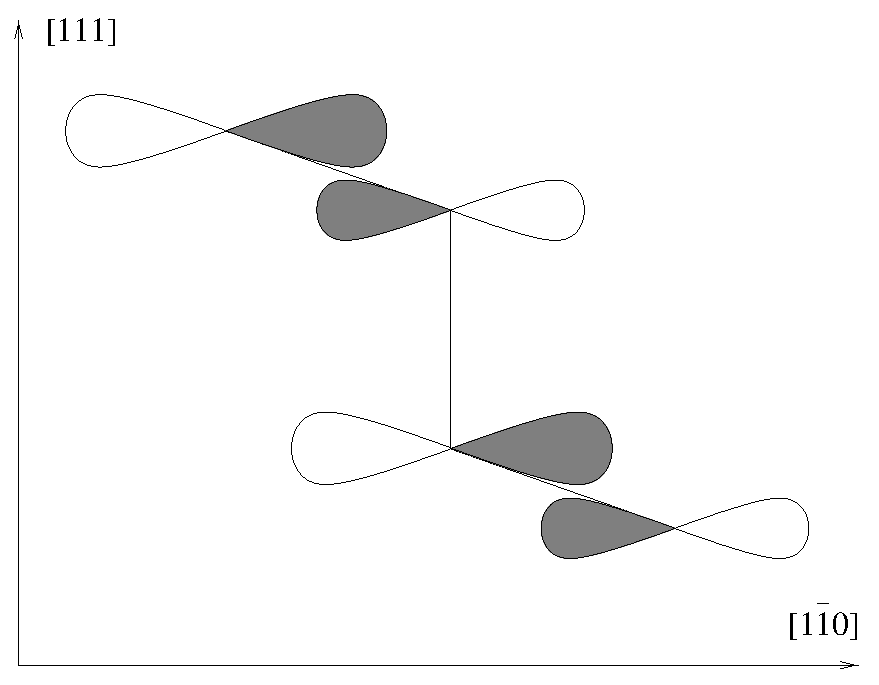
\includegraphics[width=10cm]{G5v.x.eps}\raisebox{4cm}{(b)}
  \caption{Schematische Darstellung der Wellenfunktionen von (a) \GCB\ und (b)
  \GVBx. $[1 \bar 1 0]$ entspricht der $x$-Richtung, $[111]$ der 
  $z$-Richtung. }
  \label{fig:wfkt-G}
\end{figure}
%\end{sidewaysfigure}

%\begin{sidewaysfigure}
\begin{figure}
  \centering
  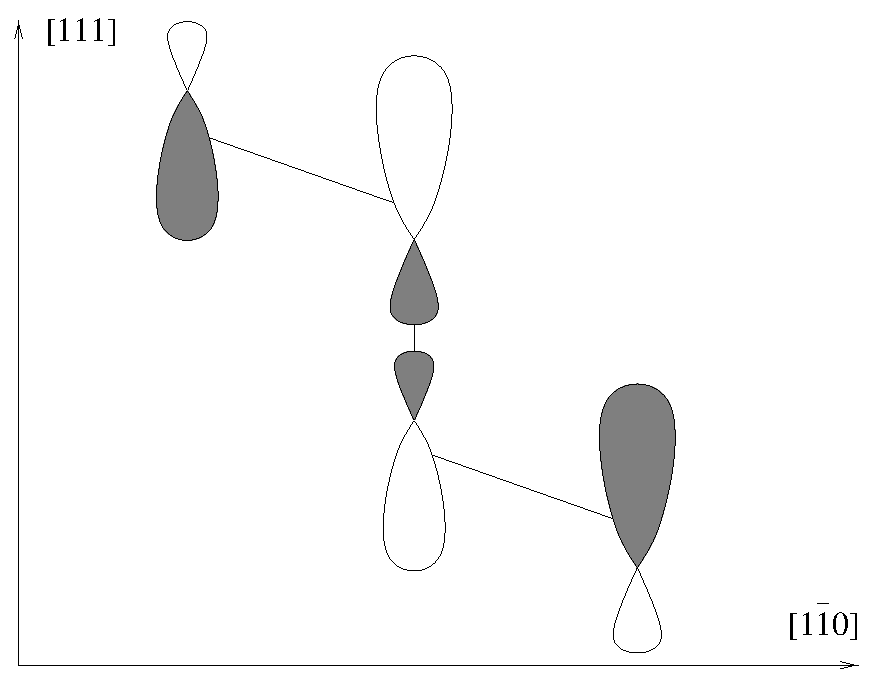
\includegraphics[width=10cm]{L1c.eps}\raisebox{4cm}{(a)}
  \vspace{2ex}
  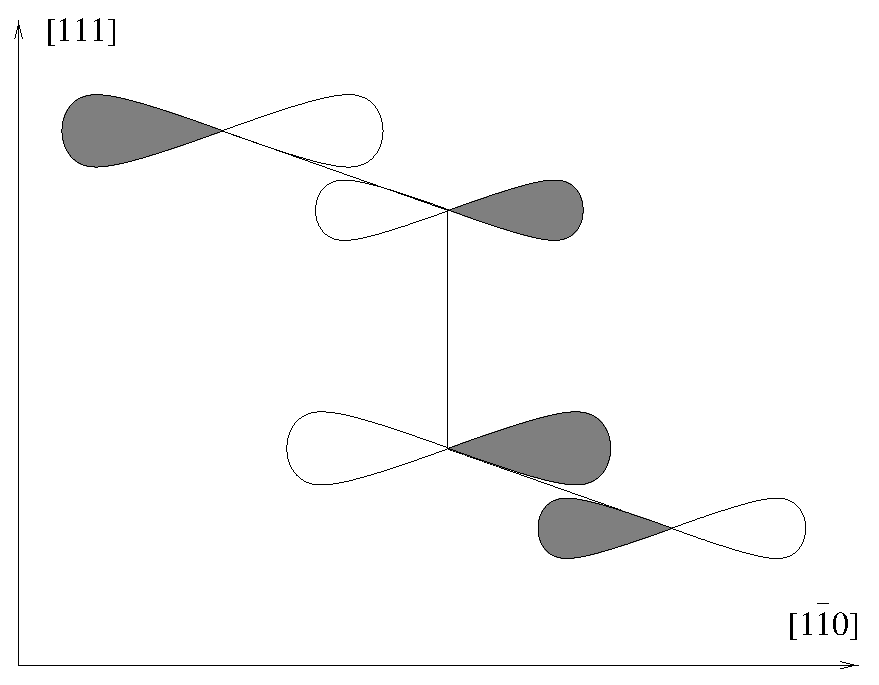
\includegraphics[width=10cm]{L3v.x.eps}\raisebox{4cm}{(b)}
  \caption{Schematische Darstellung der Wellenfunktionen von (a) \LCB\ und (b)
  \LVBx. $[1 \bar 1 0]$ entspricht der $x$-Richtung, $[111]$ der
  $z$-Richtung.}
  \label{fig:wfkt-L}
\end{figure}
%\end{sidewaysfigure}

Dadurch, da"s wir uns nun auf bestimmte Phasen der Wellenfunktionen in unserer
Basis festgelegt haben, sind im Prinzip auch die Vorzeichen der
Potentialmatrixelemente festgelegt. Doch treten dabei Schwierigkeiten auf, die
wir am Beispiel das Matrixelementes \V{35} illustrieren wollen. 

Die in Abb.~\ref{fig:wfkt-G}(b) und Abb.~\ref{fig:wfkt-L}(b) skizzierten
Valenzband-Wellenfunk"-ti"-onen lassen sich in der \CuPt-Einheitszelle als
%
\begin{subequations}
\label{eq:wfkt-tba}
\begin{eqnarray}
  \label{eq:G5v-tba}
  \ket{\GVBx} &=& -\alpha_{\Gamma} (\ket{x_{c1}} + \ket{x_{c2}})
  + \beta_{\Gamma} (\ket{x_{a1}} + \ket{x_{a2}}) \\
  \label{eq:L3v-tba}
  \ket{\LVBx} &=& +\alpha_{\text{L}} (\ket{x_{c1}} - \ket{x_{c2}}) +
  \beta_{\text{L}} (\ket{x_{a1}} - \ket{x_{a2}})
\end{eqnarray}
\end{subequations}
%
schreiben. Dabei sind $\alpha_{\Gamma}$, $\beta_{\Gamma}$, $\alpha_{\text{L}}$
und $\beta_{\text{L}}$ positive Konstanten. Die $\ket{x_{i}}$ sind auf dem
Atom $i$ [siehe Abb.~\ref{fig:wfkt-G}(a)] lokalisierte $p_{x}$-artige
Wellenfunktionen, deren positive H"alfte in positive $x$-Richtung
zeigt.\footnote{Genauer gesagt sind die $\ket{x_{i}}$ Blochsummen zu $k=0$
  "uber alle zu $i$ "aquivalente Atome im Kristall (siehe Anhang
  \ref{cha:lcao}).} 
Nun k"onnen wir den TBA-Hamilton-Operator, der den geordneten
Kristall beschreibt, in einen Teil \op{H_{0}^{\SSs \text{TBA}}}, der
Zinkblende Symmetrie besitzt, und einen Teil \op{H_{1}^{\SSs \text{TBA}}}, der
das Ordnungspotential beschreibt, aufteilen. Die Zust"ande in
Gl.~\eqref{eq:wfkt-tba} sind Eigenzust"ande von \op{H_{0}^{\SSs \text{TBA}}},
doch k"onnen wir das Matrixelement bez"uglich \op{H_{1}^{\SSs \text{TBA}}}
berechnen:
%
\begin{eqnarray}
  \label{eq:V35-tba}
  \matrixel{\GVBx}{\op{H_{1}^{\SSs \text{TBA}}}}{\LVBx} &=&
  - \alpha_{\Gamma} \alpha_{\text{L}} (\Delta E_{p}^{c1} - \Delta E_{p}^{c2})
  + \beta_{\Gamma}  \beta_{\text{L}}  (\Delta E_{p}^{a1} - \Delta E_{p}^{a2})
  \nonumber\\ && 
  - (\beta_{\text{L}}\alpha_{\Gamma} - \beta_{\Gamma} \alpha_{\text{L}}) 
    ( \Delta p_{c1}p_{a1}\pi - \Delta p_{c2}p_{a2}\pi )
  \nonumber\\ &&
  + (\beta_{\text{L}}\alpha_{\Gamma} + \beta_{\Gamma} \alpha_{\text{L}}) 
    (\frac{4}{3}(\Delta p_{c1}p_{a2}\sigma - \Delta p_{c2}p_{a1}\sigma)
  \nonumber\\ && \hspace{6.78em}
  +  \frac{5}{3}(\Delta p_{c1}p_{a2}\pi    - \Delta p_{c2}p_{a1}\pi   ) ) 
\end{eqnarray}
%
Dabei bedeutet z.~B.\ $\Delta E_{p}^{c1}$ die "Anderung in der Energie eines
$p$-Orbitals auf dem Kation C1, $\Delta p_{c1}p_{a1}\pi$ die "Anderung in der
Energie einer $pp\pi$-Bindung zwischen Kation C1 und Anion A1
etc.\footnote{Eine genauere Erkl"arung der Bedeutung dieser Parameter ist in
  Anhang~\ref{cha:lcao} zu finden.}  Um diesen Ausdruck auswerten zu k"onnen,
ben"otigen wir sowohl die Koeffizienten $\alpha_{\Gamma}$, $\beta_{\Gamma}$,
$\alpha_{\text{L}}$ und $\beta_{\text{L}}$ sowie die "Anderungen in den
Parametern der TBA. Erstere lassen sich leicht f"ur einen Satz Parameter
berechnen oder aber auch absch"atzen, da sie sich kaum zwischen verschiedenen
Kristallen mit Zinkblende-Gitter unterscheiden. Um die "Anderung in den
TBA-Parametern zu beschreiben, bieten sich die Unterschiede zwischen den
entsprechenden Parametern f"ur GaP und InP an. F"ur diese sind verschieden
Parametrisierungen durchgef"uhrt worden \cite{harr:80,chad:77,jsbb:98}, doch
sind diese Parameter abstandsabh"angig und beziehen sich auf die in GaP bzw.
InP zu findenden atomaren Abst"ande. Die atomaren Abst"ande in \GaInP\ 
entsprechen aber mehr denen in GaAs, das als Substrat w"ahrend des Wachstums
verwendet wird. Die Schwierigkeit dabei ist, da"s die Abstandsabh"angigkeit
der TBA-Parameter nicht gut bekannt ist. So werden in der Literatur sehr
verschiedene Abh"angigkeiten diskutiert \cite[p.~504ff]{jsbb:98, harr:80}.
Trotzdem k"onnen Ausdr"ucke vom Typ \eqref{eq:V35-tba} f"ur verschiedene
Parametrisierungen und Abstandsabh"angigkeiten ausgewertet werden. Doch neben
den zu erwartenden starken Unterschieden in den Betr"agen, erhalten wir auch
f"ur die Vorzeichen und die relativen Vorzeichen der Matrixelemente
verschiedene Ergebnisse, je nach dem, welche Parametrisierung wir verwenden.
Wir k"onnen aber nicht sagen, da"s eine dieser Parametrisierungen den anderen
vorzuziehen ist. Deshalb m"ussen wir folgern, da"s diese Methode nicht
geeignet ist, die relativen Vorzeichen der Potentialmatrixelemente zu
bestimmen, weshalb wir die verschiedenen M"oglichkeiten bei der Auswertung des
Hamilton-Operators \eqref{eq:k.p-H} ber"ucksichtigen m"ussen.


%%% Local Variables: 
%%% mode: latex
%%% TeX-master: "diplom"
%%% End: 



%%% Local Variables: 
%%% mode: latex
%%% TeX-master: "diplom"
%%% End: 




